\chapter{Microbiomas e simbioses}\label{ch:b3:microbiomes}

Você carrega cerca de trinta e oito trilhões de bactérias, mais ou
menos uma para cada célula sua, a maioria delas no último metro de seu
intestino, onde pesam quase tanto quanto seu cérebro e carregam cem
vezes mais genes que você. Um camundongo criado sem nenhuma delas
precisa de um terço a mais de comida para manter o peso, tem um sistema
imune atrofiado e se comporta de modo estranho. Uma ervilheira entrega
um décimo de seu açúcar a bactérias em nódulos de suas raízes e recebe
nitrogênio em troca; quatro quintos de todas as plantas terrestres
trocam açúcar por fosfato com fungos enrolados em suas raízes, como
fazem há quatrocentos milhões de anos; um coral é um animal que cultiva
algas dentro de suas células e morre quando o mar esquenta o bastante
para fazê-lo expulsá-las. Os seres vivos não são indivíduos, mas
consórcios, e este capítulo trata da biologia dessas parcerias: como
são contadas e caracterizadas por sequenciamento, o que os parceiros
trocam, como a troca é negociada e fiscalizada, e por que alguns
parceiros acabam como organelas.

\section{Palavras para conviver}

\begin{definition}[Simbiose]\label{def:b3:microbiomes:symbiosis}
\index{simbiose}\index{mutualismo}\index{comensalismo}\index{holobionte}\index{microbioma}\index{transmissão vertical}
A \emph{simbiose} é a associação sustentada e íntima de organismos de
espécies diferentes; ela é um \emph{mutualismo} se os dois ganham, um
\emph{comensalismo} se um ganha e o outro não é afetado, e um
parasitismo se um ganha às custas do outro --- e um mesmo par pode se
deslocar ao longo dessa linha conforme as circunstâncias. Um
\emph{endossimbionte} vive dentro das células de seu hospedeiro; um
parceiro \emph{obrigatório} não consegue viver sozinho. Os simbiontes
são transmitidos \emph{verticalmente}, de genitor a descendente (as
\emph{Buchnera} do pulgão passam pelo ovo), ou
\emph{horizontalmente}, adquiridos de novo a cada geração do ambiente
ou de outros hospedeiros (o \emph{Vibrio} da lula, as bactérias do
intestino humano). O \emph{microbioma} é toda a comunidade de micróbios
de um hábitat --- um intestino, a superfície de uma folha, um grama de
solo --- e o \emph{holobionte} é um hospedeiro junto com seu
microbioma, considerado como a unidade que a seleção natural enxerga.
\end{definition}

\begin{example}[Três parceiros obrigatórios]\label{ex:b3:microbiomes:obligate}
A \emph{Buchnera} do pulgão vive dentro das células de seu hospedeiro
há duzentos milhões de anos, faz os aminoácidos essenciais que faltam à
seiva do floema e encolheu seu genoma a \qty{640}{kb} --- um sétimo do
de suas parentes de vida livre ---, perdendo cada gene que o hospedeiro
agora fornece. A bactéria \emph{Wolbachia}, presente em dois terços das
espécies de insetos, é transmitida só pelos ovos e por isso evoluiu
para favorecer as fêmeas: ela mata embriões machos, feminiza-os, ou faz
os ovos de fêmeas não infectadas morrerem quando fecundados por machos
infectados (a \emph{incompatibilidade citoplasmática}), o que a espalha
por uma população; mosquitos que a carregam transmitem mal a dengue, e
soltá-los reduziu a dengue em várias cidades. A ameba
\emph{Paulinella} acolheu uma cianobactéria há cerca de cem milhões de
anos, que hoje não é bem uma bactéria nem bem um cloroplasto --- uma
segunda origem independente de organelas fotossintéticas, apanhada no
meio do caminho.
\end{example}

\section{Contar uma comunidade}

\begin{method}[Perfilar um microbioma por sequenciamento]\label{met:b3:microbiomes:16s}
\index{sequenciamento do 16S rRNA}\index{metagenômica}\index{unidade taxonômica operacional}
A maioria dos micróbios não pode ser cultivada; eles são contados por
seu DNA. (1) Extraia o DNA da amostra --- fezes, solo, água do mar
filtrada numa membrana. (2) Ou amplifique o gene do RNA ribossômico da
subunidade pequena (o \emph{16S}) com \omterm{def:b3:genetic-engineering:pcr}{iniciadores} que correspondam a
suas regiões universais, e sequencie as regiões variáveis entre elas
--- um levantamento de \emph{amplicons}, barato, que identifica
bactérias até mais ou menos o gênero e as conta pelo número de leituras;
ou sequencie todo o DNA --- a \emph{metagenômica aleatória}, que
recupera genes e genomas inteiros e assim relata o que a comunidade
sabe fazer, e não apenas quem está lá. (3) Agrupe as leituras em
variantes de sequência ou em \emph{\omterm{met:b3:microbiomes:16s}{unidades taxonômicas operacionais}}
(OTUs, convencionalmente a \qty{97}{\%} de identidade para uma
``espécie''), atribua-as por comparação com bancos de dados
(\cref{ch:b3:bioinformatics}) e tabule as contagens por amostra. (4)
Calcule a diversidade dentro de uma amostra e compare a composição
entre amostras. As contagens são relativas --- as leituras de uma
amostra somam um total fixo --- e são enviesadas pela extração, pelos
\omterm{def:b3:genetic-engineering:pcr}{iniciadores} e pelo número de cópias, de modo que as diferenças entre
amostras processadas do mesmo modo são confiáveis onde os números
absolutos não são.
\end{method}

\begin{definition}[Diversidade]\label{def:b3:microbiomes:diversity}
\index{riqueza de espécies}\index{índice de Shannon}\index{índice de Simpson}\index{rarefação}
Para uma comunidade de $S$ espécies com abundâncias relativas
$p_{1},\dots,
p_{S}$ ($\sum p_{i} = 1$): a \emph{riqueza} é $S$; o
\emph{índice de Shannon} $H = -\sum_{i} p_{i}\ln p_{i}$ mede a
incerteza sobre a espécie de um indivíduo sorteado ao acaso, e $e^{H}$
é o número de espécies igualmente abundantes que daria a mesma
incerteza (o número efetivo de espécies); o \emph{índice de Simpson}
$D = \sum_{i} p_{i}^{2}$ é a probabilidade de dois indivíduos sorteados
ao acaso serem da mesma espécie, e $1/D$ é outro número efetivo,
ponderado a favor das espécies comuns. A riqueza depende de quantos
indivíduos se examinou: uma \emph{curva de rarefação} representa as
espécies encontradas contra o número de indivíduos amostrados, e se
achata quando a maioria das espécies já foi vista.
\end{definition}

\begin{theorem}[Rarefação]\label{thm:b3:microbiomes:rarefaction}
\index{rarefação!fórmula}\index{cobertura de Good}
Uma amostra contém $N$ indivíduos de $S$ espécies, $N_{i}$ da espécie
$i$. O número esperado de espécies numa subamostra aleatória de $n$
indivíduos, sorteada sem reposição, é
\[
E[S_{n}] = \sum_{i=1}^{S}\left[1 - \frac{\binom{N - N_{i}}{n}}
{\binom{N}{n}}\right],
\]
que sobe com $n$ e vale $S$ em $n = N$. Duas amostras de tamanhos
diferentes são comparadas rarefazendo as duas ao mesmo $n$. A fração
dos indivíduos da comunidade que pertencem a espécies ainda não vistas
é estimada pela \emph{\omterm{thm:b3:microbiomes:rarefaction}{cobertura de Good}}: cerca de $f_{1}/N$, em que
$f_{1}$ é o número de espécies vistas exatamente uma vez (os
singletons).
\end{theorem}
\begin{proof}
A espécie $i$ está ausente da subamostra exatamente quando todos os $n$
indivíduos são sorteados entre os $N - N_{i}$ outros, o que acontece em
$\binom{N - N_{i}}{n}$ das $\binom{N}{n}$ subamostras igualmente
prováveis; logo a espécie $i$ está presente com probabilidade
$1 - \binom{N-N_{i}}{n}/
\binom{N}{n}$, e a contagem esperada de espécies
presentes é a soma dessas probabilidades (a esperança de uma soma de
indicadores). Cada termo cresce com $n$, e em $n = N$ todo binomial do
numerador é zero. A estimativa de Good: um indivíduo sorteado a seguir
pertence a uma espécie não vista com mais ou menos a probabilidade de
um indivíduo sorteado ao acaso da amostra ser o único de seu tipo,
$f_{1}/N$ (Good, 1953); sua justificativa é aqui admitida.
\end{proof}

\begin{example}[Dois intestinos]\label{ex:b3:microbiomes:two-guts}
Uma amostra de $1000$ leituras de uma pessoa dá $150$ espécies, com
$H = 3.5$ e $40$ singletons; uma amostra de $5000$ leituras de outra dá
$260$ espécies. A segunda não é necessariamente mais diversa: ela foi
amostrada cinco vezes mais a fundo, e rarefazê-la a $1000$ leituras
pode dar $150$ também. A cobertura da primeira amostra é
$1 - 40/1000 =
\qty{96}{\%}$: quatro por cento das bactérias daquele
intestino pertencem a espécies que a amostra nunca viu, e uma amostra
mais profunda as encontrará. Os números efetivos --- $e^{3.5} \approx 33$ espécies em equitatividade contra uma riqueza de $150$ --- dizem
que umas poucas espécies dominam, que é como todo intestino se
apresenta.
\end{example}

\begin{omfigure}
\begin{tikzpicture}
\begin{axis}[
  width=0.68\linewidth, height=5.6cm,
  axis x line=bottom, axis y line=left,
  xmin=0, xmax=5000, ymin=0, ymax=300,
  xlabel={leituras amostradas, $n$}, ylabel={espécies observadas},
  xlabel style={font=\small, at={(axis description cs:0.5,-0.12)}, anchor=north}, ylabel style={font=\small},
  tick label style={font=\small}, xtick={0,1000,2000,3000,4000,5000}, ytick={0,100,150,200,260},
  clip=false,
]
\addplot[very thick, omDef, domain=0:5000, samples=60] {260*(1-exp(-x/1500))};
\addplot[very thick, omThm, domain=0:1000, samples=30] {150*(1-exp(-x/300))*1.0};
\addplot[very thick, omThm, dashed, domain=1000:5000, samples=30] {150*(1-exp(-x/300))*1.0 + 8*(1-exp(-(x-1000)/2000))};
\draw[dashed, gray] (axis cs:1000,0) -- (axis cs:1000,300);
\node[font=\scriptsize, omDef, anchor=north west] at (axis cs:1200,292) {segundo intestino: $260$ espécies em $5000$ leituras};
\node[font=\scriptsize, omThm, anchor=north east] at (axis cs:4900,140) {primeiro intestino: $150$ em $1000$, perto de seu platô};
\node[font=\scriptsize, gray, anchor=south west] at (axis cs:1050,10) {rarefaça aqui para comparar};
\end{axis}
\end{tikzpicture}

{\small Curvas de \omterm{def:b3:microbiomes:diversity}{rarefação}. As espécies encontradas sobem com as
leituras amostradas e se achatam à medida que a comunidade se esgota;
duas amostras são comparadas na mesma profundidade. Aqui o segundo
intestino ainda está subindo em $5000$ leituras, de modo que sua riqueza
verdadeira é ainda maior.}
\end{omfigure}

\section{O microbioma humano}

\begin{definition}[A comunidade do intestino]\label{def:b3:microbiomes:gut}
\index{microbioma intestinal}\index{ácido graxo de cadeia curta}\index{resistência à colonização}\index{disbiose}
O intestino humano abriga cerca de $4\times 10^{13}$ bactérias, quase
todas no cólon, a $10^{11}$ por grama de conteúdo, contra $10^{3}$ por
grama no estômago ácido e $10^{4}$--$10^{7}$ ao longo do intestino
delgado, cujo fluxo é rápido e cuja bile é hostil. Umas quinhentas a
mil espécies por pessoa, a maioria de dois filos, os Bacteroidetes e os
Firmicutes, quase todas anaeróbias; o conjunto de cada pessoa é
distinto e estável por anos, fixado em grande parte nos três primeiros
anos de vida a partir da mãe e da casa. O que elas fazem: fermentam a
fibra que as enzimas humanas não digerem em \emph{ácidos graxos de
cadeia curta} --- acetato, propionato, butirato ---, que alimentam as
próprias células do cólon e fornecem até um décimo das calorias do
hospedeiro; produzem vitamina~K e algumas vitaminas do complexo B;
transformam ácidos biliares e fármacos; ocupam cada nicho, de modo que
um invasor não encontra apoio (a \emph{resistência à colonização}); e
treinam o sistema imune, cujos linfócitos~T reguladores e células
secretoras de IgA se desenvolvem em resposta a elas
(\cref{ch:b3:adaptive-immunity}). Uma comunidade afastada desse estado
--- menos espécies, menos fermentadoras, mais aeróbias facultativas ---
é uma \emph{disbiose}, vista na doença inflamatória intestinal, depois
de \omterm{def:b3:bacteriology:antibiotics}{antibióticos} e na obesidade, embora em geral não esteja claro o que
é causa e o que é efeito.
\end{definition}

\begin{proof}[Evidência]
Camundongos criados livres de germes em isoladores estéreis (Gordon e
colaboradores, anos 2000) têm paredes intestinais finas, órgãos
linfoides pequenos, níveis baixos de anticorpos e precisam de
\qty{30}{\%} mais calorias para manter o peso; colonizados com uma
microbiota normal de camundongo, ganham gordura em duas semanas.
Recebendo a microbiota de um camundongo obeso em vez da de um magro,
camundongos livres de germes ganharam mais gordura com a mesma comida
(Turnbaugh, 2006): a própria comunidade afeta a colheita de energia.
Nos humanos, a colite recorrente por \emph{Clostridioides difficile}
--- uma \omterm{def:b3:microbiomes:gut}{disbiose} em que os \omterm{def:b3:bacteriology:antibiotics}{antibióticos} removeram os concorrentes de um
esporulador produtor de toxina --- foi curada em \qty{94}{\%} dos
pacientes pela infusão das fezes de um doador saudável, contra
\qty{31}{\%} com o \omterm{def:b3:bacteriology:antibiotics}{antibiótico} padrão (van~Nood, 2013), o primeiro
ensaio randomizado em que o fármaco foi uma comunidade, e não uma
molécula.
\end{proof}

\begin{omfigure}
\begin{tikzpicture}
\begin{axis}[
  width=0.68\linewidth, height=5.4cm,
  ybar, bar width=18pt,
  axis x line=bottom, axis y line=left,
  ymode=log, ymin=1, ymax=1e13,
  symbolic x coords={stomach, duodenum, jejunum, ileum, colon},
  xtick=data, xticklabels={estômago, duodeno, jejuno, íleo, cólon}, ytick={1e1,1e3,1e5,1e7,1e9,1e11},
  ylabel={bactérias por grama de conteúdo},
  ylabel style={font=\small}, tick label style={font=\small},
  clip=false,
]
\addplot[fill=omDef!40, draw=omDef] coordinates {(stomach,1e3) (duodenum,1e4) (jejunum,1e5) (ileum,1e7) (colon,1e11)};
\node[font=\scriptsize, anchor=west, xshift=10pt] at (axis cs:stomach,3e3) {ácido, pH 2};
\node[font=\scriptsize, anchor=south] at (axis cs:jejunum,1.5e5) {bile, fluxo rápido};
\node[font=\scriptsize, anchor=south, align=center] at (axis cs:colon,1.5e11) {lento, anaeróbio:\\o fermentador};
\end{axis}
\end{tikzpicture}

{\small Densidade bacteriana ao longo do intestino humano, em escala
logarítmica: uma subida de cem milhões de vezes do estômago ácido até o
cólon, onde vivem quase todos os micróbios do corpo.}
\end{omfigure}

\begin{omfigure}
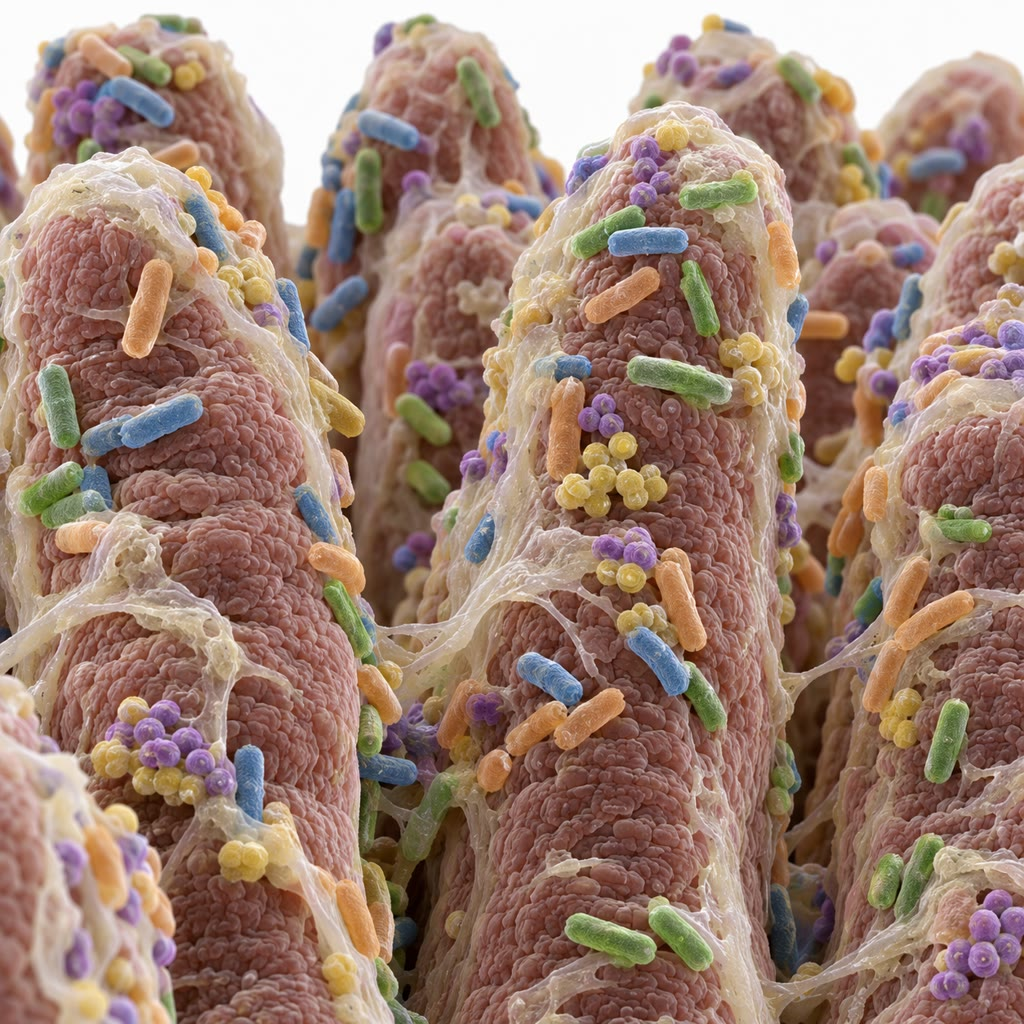
\includegraphics[width=0.40\linewidth]{images/book5/ai/b5-14-gut-microbiota.jpg}

{\small A superfície do revestimento intestinal no microscópio
eletrônico de varredura, com bactérias de vários tipos alojadas no muco
entre as vilosidades.}
\end{omfigure}

\section{As plantas e seus parceiros}

\begin{definition}[A simbiose leguminosa--rizóbio]\label{def:b3:microbiomes:nodule}
\index{rizóbios}\index{nódulo radicular}\index{fator Nod}\index{leghemoglobina}\index{nitrogenase}
As leguminosas abrigam bactérias fixadoras de nitrogênio (os
\emph{rizóbios}) em \emph{nódulos radiculares}, órgãos construídos para
isso depois de um diálogo molecular. A raiz secreta flavonoides; um
rizóbio da espécie correspondente responde com \emph{fatores Nod} ---
lipoquito-oligossacarídeos cujos ornamentos especificam o parceiro; uma
cinase receptora do pelo radicular os liga e dispara oscilações de
cálcio no núcleo, o encurvamento do pelo em torno das bactérias e um
\emph{cordão de infecção} que cresce para dentro através das células,
enquanto o córtex abaixo começa a se dividir num nódulo. As bactérias
são liberadas nas células do nódulo dentro de membranas e se
diferenciam em \emph{bacteroides} que expressam a \emph{nitrogenase}, a
enzima que reduz o N$_{2}$ a amônia ao custo de dezesseis ATP por
molécula. A nitrogenase é destruída pelo oxigênio, e ainda assim os
bacteroides respiram muito; o nódulo resolve a contradição com uma
barreira de difusão e com a \emph{leghemoglobina}, uma hemoglobina
vegetal que liga o oxigênio com força e o entrega aos bacteroides numa
concentração livre baixa --- é ela que faz um nódulo cortado ser rosa.
A planta paga de seis a dez por cento de seu fotossintato e recebe a
maior parte de seu nitrogênio; o nitrogênio fixado pelas leguminosas
cultivadas no mundo se aproxima do da indústria de fertilizantes.
\end{definition}

\begin{omfigure}
\begin{tikzpicture}[every node/.style={font=\scriptsize}, >=stealth]
  % stage 1: root hair and bacteria, flavonoid / Nod factor exchange
  \begin{scope}
    \draw[thick, omMeth!60!black, fill=omMeth!15] (0,0) rectangle (1.2,3.0);
    \draw[thick, omMeth!60!black, fill=omMeth!15] (1.2,1.6) .. controls (2.4,1.7) and (2.6,2.6) .. (2.9,2.4) .. controls (2.5,2.3) and (2.3,1.4) .. (1.2,1.2) -- cycle;
    \foreach \p in {(3.1,2.7),(3.4,2.3),(3.3,1.9)} \fill[omProp] \p ellipse (0.14 and 0.07);
    \draw[->, omMeth!60!black, thick] (2.6,1.5) -- (3.2,1.4); \node[below, omMeth!60!black] at (3.0,1.35) {flavonoides};
    \draw[<-, omProp, thick] (2.5,2.85) -- (3.0,3.0); \node[above, omProp] at (2.4,2.95) {fatores Nod};
    \node[below, align=center] at (1.6,-0.2) {1. diálogo: pelo radicular\\e rizóbios};
  \end{scope}
  % stage 2: curled hair, infection thread
  \begin{scope}[xshift=4.6cm]
    \draw[thick, omMeth!60!black, fill=omMeth!15] (0,0) rectangle (1.2,3.0);
    \draw[thick, omMeth!60!black, fill=omMeth!15] (1.2,1.6) .. controls (2.3,1.8) and (2.8,2.6) .. (2.2,2.8) .. controls (1.9,2.9) and (1.8,2.5) .. (2.0,2.4) .. controls (2.3,2.2) and (1.9,1.3) .. (1.2,1.2) -- cycle;
    \draw[omProp, very thick] (2.05,2.55) .. controls (1.8,2.1) and (1.4,1.7) .. (0.4,1.3);
    \foreach \p in {(1.85,2.3),(1.5,1.9),(1.1,1.6),(0.7,1.4)} \fill[omProp] \p ellipse (0.1 and 0.05);
    \node[right, omProp, font=\tiny] at (2.3,1.0) {cordão de infecção};
    \foreach \p in {(0.3,0.5),(0.6,0.7),(0.9,0.5)} \draw[omMeth!60!black] \p circle (0.12);
    \node[below, align=center] at (1.6,-0.2) {2. o pelo se encurva; o cordão entra;\\as células do córtex se dividem};
  \end{scope}
  % stage 3: nodule
  \begin{scope}[xshift=9.0cm]
    \draw[thick, omMeth!60!black, fill=omMeth!15] (0,0) rectangle (1.2,3.0);
    \draw[thick, omThm!60!black, fill=omThm!25] (1.2,1.5) ellipse (1.3 and 1.0);
    \foreach \p in {(1.0,1.5),(1.5,1.8),(1.6,1.2),(1.1,1.9),(1.2,1.1),(2.0,1.5)} \fill[omProp] \p circle (0.1);
    \node[right, align=left] at (2.6,2.0) {nódulo: bacteroides\\com nitrogenase};
    \node[right, align=left, omThm!60!black] at (2.6,1.1) {rosa: a leghemoglobina\\mantém o O$_2$ baixo};
    \draw[->, thick] (0.6,2.4) -- (1.0,2.0) node[pos=0, above] {açúcar};
    \draw[<-, thick] (0.6,0.6) -- (1.0,1.0) node[pos=0, below] {NH$_3$};
    \node[below, align=center] at (1.6,-0.2) {3. os bacteroides fixam N$_2$;\\açúcar por amônia};
  \end{scope}
\end{tikzpicture}

{\small Fazer um nódulo. Os flavonoides da raiz e os \omterm{def:b3:microbiomes:nodule}{fatores Nod} do
rizóbio identificam os parceiros; o pelo radicular se encurva, um
cordão de infecção leva as bactérias para dentro, e o córtex constrói
um nódulo em que os bacteroides, mantidos em baixo oxigênio pela
\omterm{def:b3:microbiomes:nodule}{leghemoglobina}, fixam nitrogênio em troca de açúcar.}
\end{omfigure}

\begin{definition}[Micorrizas]\label{def:b3:microbiomes:mycorrhiza}
\index{micorriza}\index{micorriza arbuscular}\index{via comum da simbiose}
As \emph{micorrizas} são associações de raízes com fungos, encontradas
em uns \qty{80}{\%} das espécies vegetais e nos fósseis mais antigos de
plantas terrestres. Nas \emph{micorrizas arbusculares} o fungo entra
nas células da raiz e se ramifica num arbúsculo em forma de árvore,
através do qual fosfato, nitrogênio e água passam à planta, e açúcares
e lipídios ao fungo; as hifas fúngicas estendem cem vezes a superfície
de absorção da raiz e alcançam fosfato que a raiz não alcança. Nas
\emph{ectomicorrizas}, das árvores de floresta, o fungo embainha a raiz
e cresce entre as células. Os genes vegetais que admitem o fungo são a
mesma \emph{via comum da \omterm{def:b3:microbiomes:symbiosis}{simbiose}} --- receptor, picos de cálcio,
fatores de transcrição --- que as leguminosas reaproveitam para os
\omterm{def:b3:microbiomes:nodule}{rizóbios}: o nódulo é uma invenção tardia construída sobre uma parceria
fúngica quatrocentos milhões de anos mais velha.
\end{definition}

\begin{proposition}[O comércio e sua fiscalização]\label{prop:b3:microbiomes:sanctions}
\index{escolha de parceiro}\index{sanções}\index{trapaceiro}
Um \omterm{def:b3:microbiomes:symbiosis}{mutualismo} é uma troca, e cada parceiro é selecionado para dar menos
e receber mais; ele persiste porque o outro parceiro pode retaliar. As
leguminosas restringem o oxigênio aos nódulos cujos \omterm{def:b3:microbiomes:nodule}{rizóbios} não fixam
nitrogênio, reduzindo à metade sua reprodução (Kiers, 2003): as
\emph{sanções}. As plantas em redes micorrízicas destinam mais carbono
aos parceiros fúngicos que entregam mais fosfato, e os fungos mais
fosfato às raízes que pagam mais carbono --- um mercado em que os dois
lados recompensam o melhor negociante (Kiers, 2011). As lulas expelem
as bactérias do órgão de luz que não brilham; os sistemas imunes
humanos toleram os comensais que ficam no lúmen e atacam os que cruzam
a parede. Onde um hospedeiro não pode nem escolher nem sancionar --- um
endossimbionte herdado pelo ovo ---, o \omterm{def:b3:bioinformatics:alignment}{alinhamento} de interesses vem,
em vez disso, do destino compartilhado: um simbionte de \omterm{def:b3:microbiomes:symbiosis}{transmissão
vertical} só se reproduz quando seu hospedeiro se reproduz, e a seleção
sobre o simbionte favorece a reprodução do hospedeiro. O modo de
transmissão, assim, prevê o caráter da parceria: a \omterm{def:b3:microbiomes:symbiosis}{transmissão vertical}
rumo ao \omterm{def:b3:microbiomes:symbiosis}{mutualismo} e à dependência, e a horizontal rumo à exploração
contida pela fiscalização.
\end{proposition}
\admitted

\begin{omfigure}
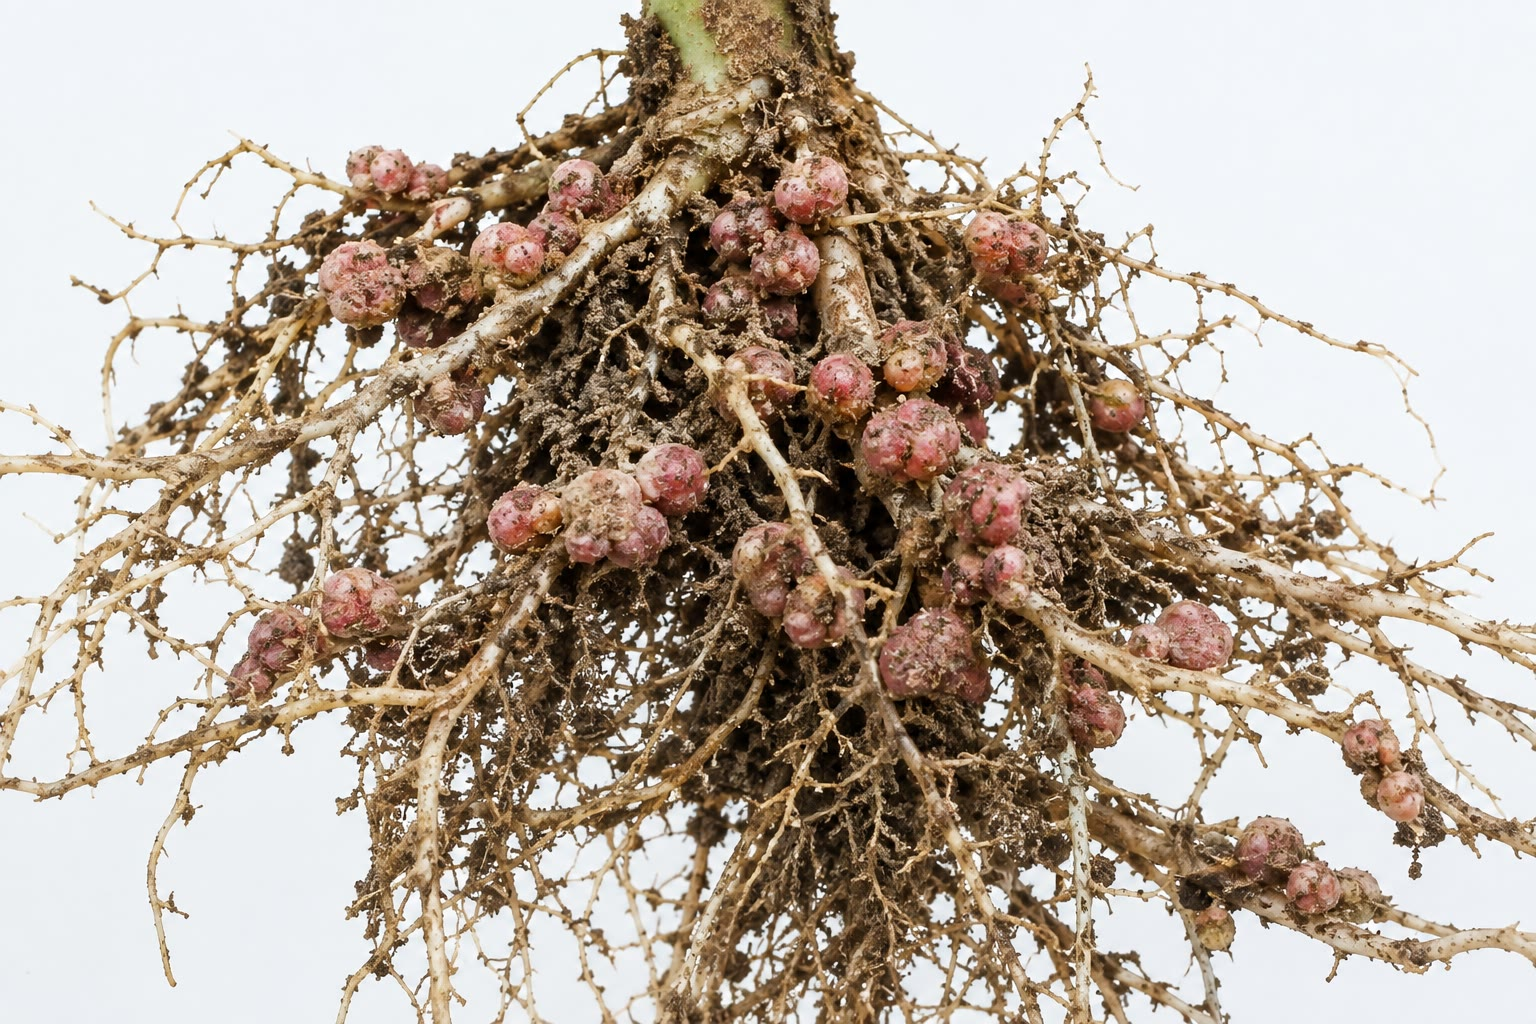
\includegraphics[width=0.46\linewidth]{images/book5/ai/b5-14-root-nodules.jpg}\hspace{0.04\linewidth}
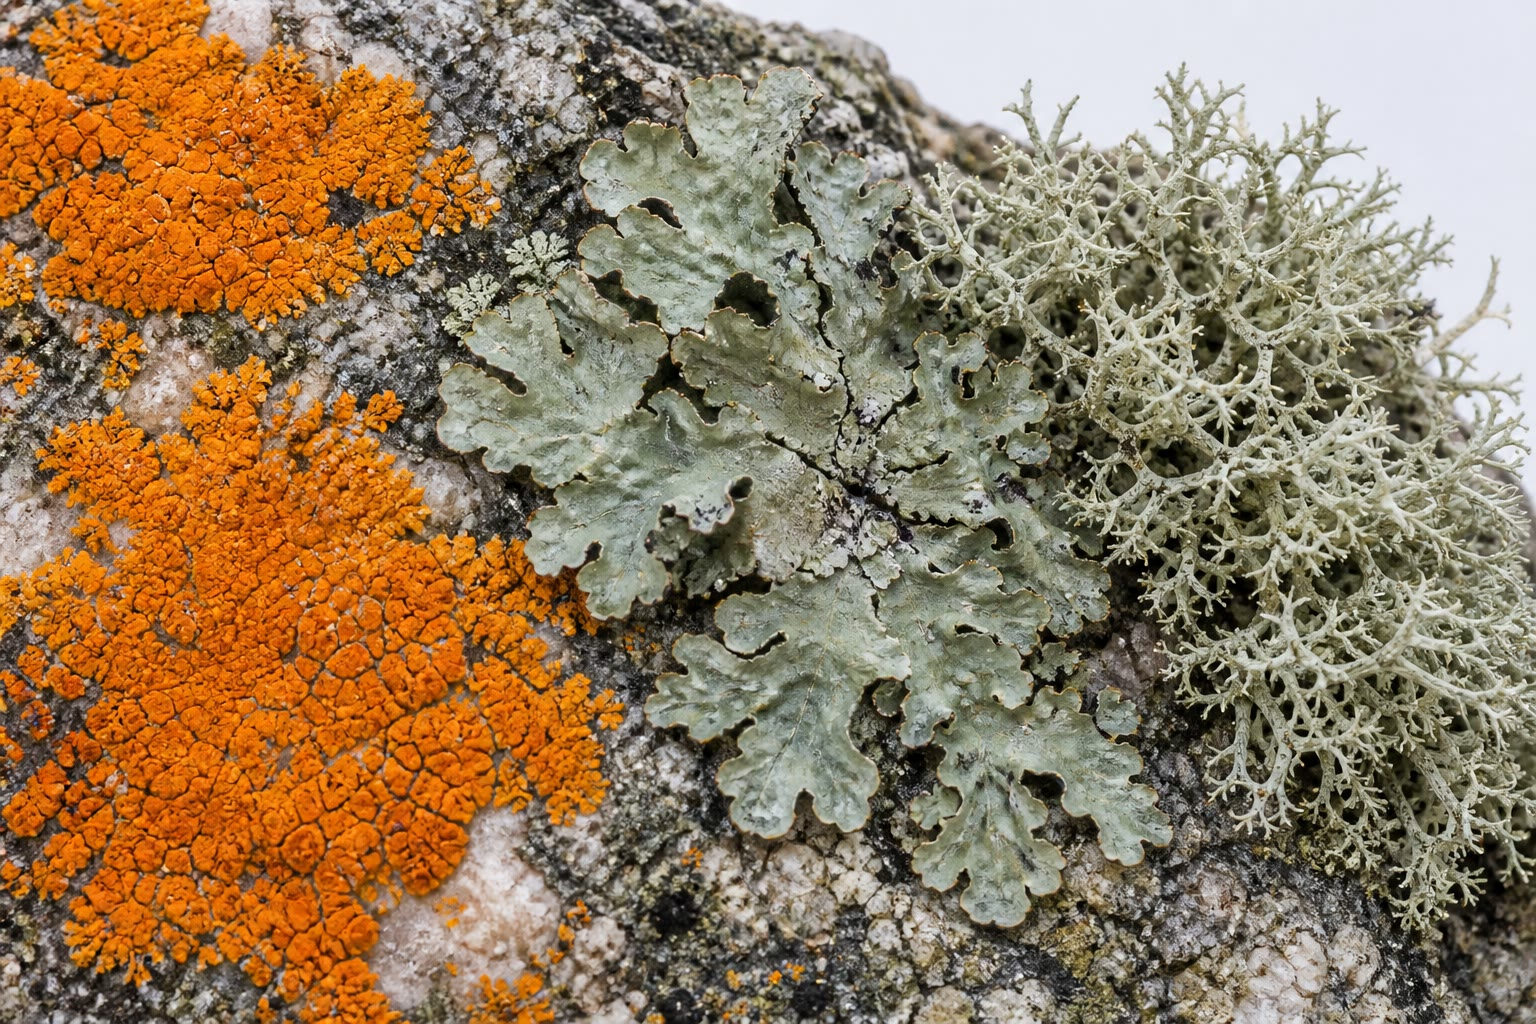
\includegraphics[width=0.46\linewidth]{images/book5/ai/b5-14-lichen.jpg}

{\small À esquerda: as raízes noduladas de uma leguminosa, cada nódulo
rosa uma fábrica de nitrogênio de bacteroides alimentada com açúcar. À
direita: liquens sobre rocha --- cada um um fungo que abriga uma alga
fotossintética ou uma cianobactéria, colonizando juntos uma superfície
que nenhum dos dois manteria sozinho.}
\end{omfigure}

\section{Parcerias no mar e em outros lugares}

\begin{definition}[O coral e a alga]\label{def:b3:microbiomes:coral}
\index{simbiose dos corais}\index{zooxantelas}\index{branqueamento dos corais}
Os corais construtores de recifes abrigam algas dinoflageladas (as
\emph{Symbiodiniaceae}, as \emph{zooxantelas}) dentro das células do
revestimento de seu intestino, um milhão ou mais por centímetro
quadrado. As algas fazem fotossíntese no tecido do animal, usando o
CO$_{2}$, a amônia e o fosfato de resíduo do animal, e devolvem até
\qty{90}{\%} do carbono que fixam como glicerol, açúcares e
aminoácidos, que alimentam o coral e a calcificação que constrói o
recife; o coral, por sua vez, controla o suprimento de nitrogênio das
algas e, com isso, seu crescimento. A parceria funciona dentro de uma
janela térmica estreita: quando a água fica cerca de um a dois graus
acima do máximo de verão por algumas semanas, a fotossíntese das algas
é danificada, elas liberam oxigênio reativo nas células hospedeiras e o
coral as expulsa --- o \emph{branqueamento}, com o esqueleto branco
aparecendo através do animal translúcido. Um coral branqueado passa
fome; ele se recupera se a água esfriar em poucas semanas, e morre se
não esfriar. A frequência do branqueamento subiu cinco vezes desde
1980, e é o mecanismo pelo qual o aquecimento está removendo os
recifes.
\end{definition}

\begin{example}[Simbioses que fazem hábitats]\label{ex:b3:microbiomes:habitats}
Um \emph{líquen} é um fungo que abriga uma alga verde ou uma
cianobactéria, com o fungo fornecendo estrutura, retenção de água e
minerais dissolvidos da rocha, e o fotobionte fornecendo açúcar (e, se
for uma cianobactéria, nitrogênio); os liquens cobrem cerca de
\qty{8}{\%} da superfície terrestre, colonizam rocha nua e começam sua
conversão em solo. O verme tubícola \emph{Riftia} das fontes
hidrotermais profundas não tem boca nem intestino quando adulto; ele
abriga bactérias oxidadoras de sulfeto num trofossomo e lhes entrega
sulfeto e oxigênio numa hemoglobina que liga os dois, crescendo mais de
um metro por ano no escuro, com energia química. Os cupins digerem
madeira com uma comunidade intestinal de protistas e bactérias, e os
ruminantes digerem capim com um rúmen do tamanho de uma banheira em que
bactérias, arqueias e fungos fermentam a celulose em ácidos graxos e
metano; a vaca vive dos ácidos graxos e dos corpos dos próprios
micróbios. Em cada caso, uma capacidade metabólica --- fotossíntese,
fixação de nitrogênio, oxidação de sulfeto, digestão de celulose --- que
a linhagem hospedeira nunca evoluiu foi adquirida por parceria numa
única etapa.
\end{example}

\begin{omfigure}
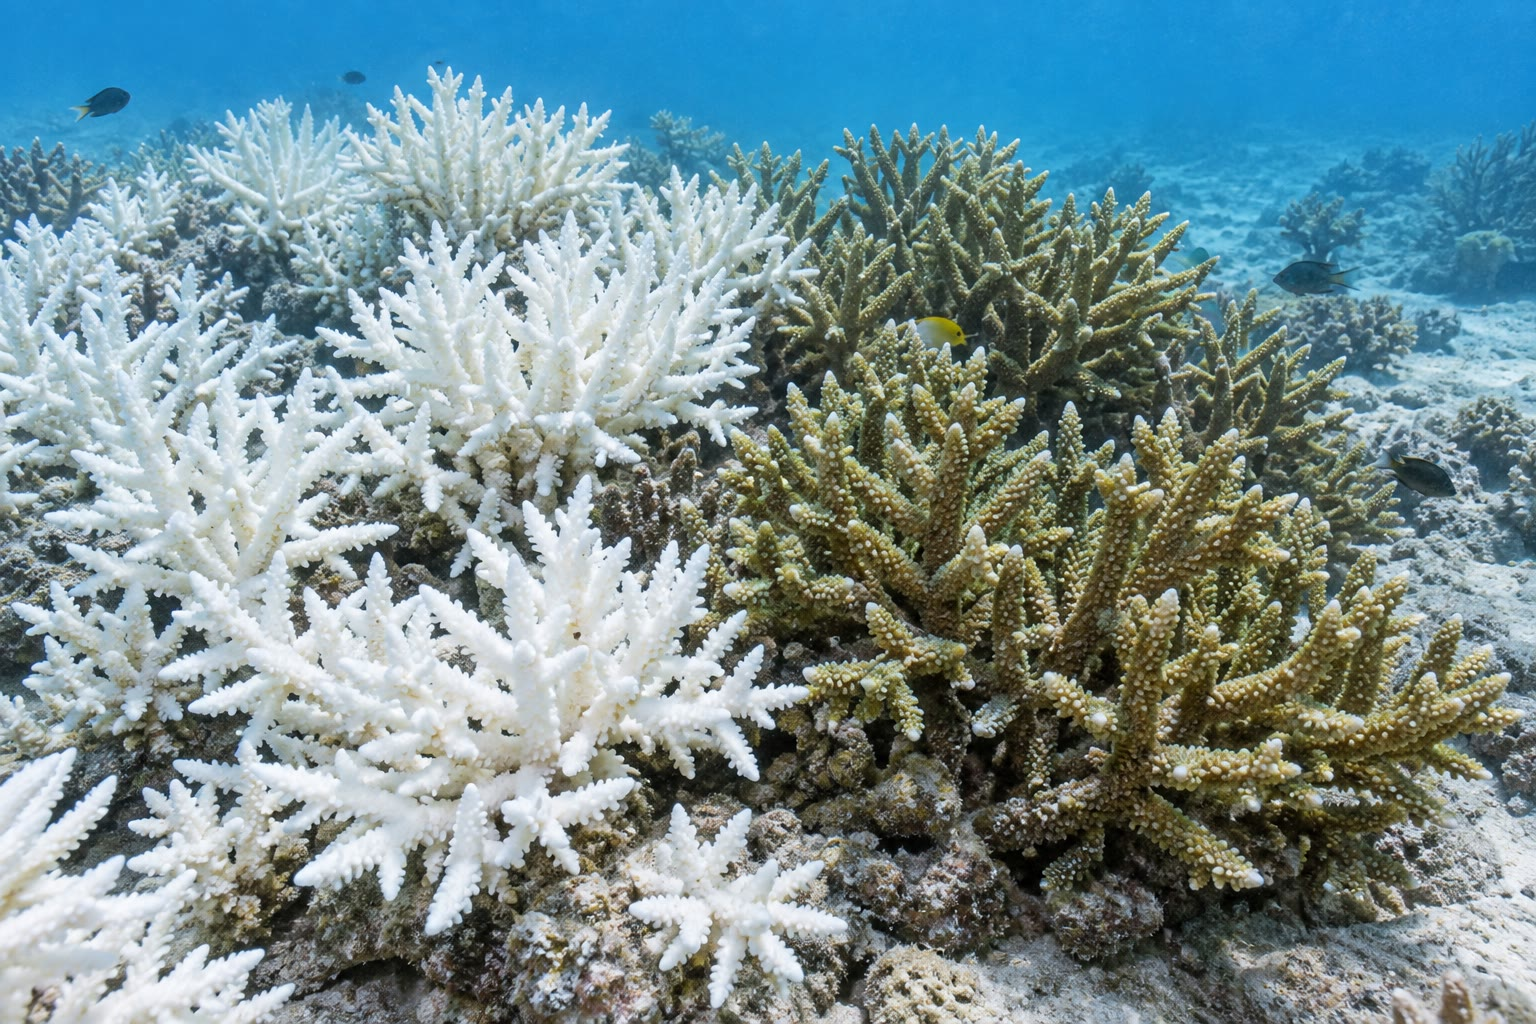
\includegraphics[width=0.56\linewidth]{images/book5/ai/b5-14-coral-bleaching.jpg}

{\small Um recife metade branqueado: as colônias brancas expulsaram
suas algas depois de semanas de água quente demais; as marrons ainda
conservam as suas. O coral branco está vivo e passando fome, e tem
semanas para ser recolonizado.}
\end{omfigure}

\begin{omfigure}
\begin{tikzpicture}[every node/.style={font=\scriptsize}, >=stealth]
  % coral cell with alga
  \draw[very thick, omDef, fill=omDef!8] (0,0) ellipse (3.2 and 2.0); \node[above] at (0,2.05) {célula do coral (gastroderme)};
  \draw[thick, omMeth!70!black, fill=omMeth!30] (-0.4,-0.1) circle (1.05); \node[align=center] at (-0.4,-0.1) {alga\\(zooxantela)};
  % exchanges
  \draw[->, thick, omMeth!70!black] (0.5,0.4) -- (1.9,0.9) node[right, align=left] {glicerol, açúcares, aminoácidos:\\até \qty{90}{\%} do carbono fixado};
  \draw[<-, thick, omThm] (0.5,-0.5) -- (1.9,-1.0) node[right, align=left] {CO$_2$, NH$_3$, fosfato\\(os resíduos do animal)};
  \draw[<-, thick, omProp] (-1.3,0.3) -- (-2.6,1.0) node[left, align=right] {luz através\\do tecido};
  \node[below, align=center] at (1.5,-2.1) {estresse: água quente por semanas $\to$ fotossíntese danificada,\\oxigênio reativo $\to$ alga expulsa $\to$ branqueamento};
  % thermometer-like bar on the right
  \begin{scope}[xshift=7.6cm, yshift=-1.6cm]
    \draw[thick] (0,0) rectangle (0.5,3.2);
    \fill[omDef!40] (0,0) rectangle (0.5,2.0); \fill[omProp!60] (0,2.0) rectangle (0.5,2.6); \fill[omThm!60] (0,2.6) rectangle (0.5,3.2);
    \node[right] at (0.6,1.0) {faixa normal}; \node[right] at (0.6,2.3) {$+\qty{1}{\celsius}$: estresse}; \node[right, align=left] at (0.6,2.9) {$+\qty{2}{\celsius}$ por semanas:\\branqueamento};
    \node[below, align=center] at (0.25,-0.1) {temperatura do mar\\no verão};
  \end{scope}
\end{tikzpicture}

{\small A troca coral--alga: a alga fixa carbono com os resíduos do
animal e com a luz que atravessa seu tecido, e devolve a maior parte
dele como alimento; uma elevação pequena e sustentada da temperatura
rompe a parceria.}
\end{omfigure}

\section{De parceiro a organela}

\begin{proposition}[Redução do genoma e o caminho até a organela]\label{prop:b3:microbiomes:reduction}
\index{redução do genoma}\index{transferência gênica endossimbiótica}
Um endossimbionte herdado pelo ovo vive numa população de algumas
poucas células que nunca recombinam com forasteiras. A seleção sobre
ele é fraca (\cref{ch:b3:molecular-evolution}: uma população pequena
fixa por deriva mutações levemente danosas), os genes cujos produtos o
hospedeiro fornece não fazem falta quando quebram, e um gene perdido
nunca é reavido. O genoma, portanto, encolhe geração após geração --- a
\emph{Buchnera} a \qty{640}{kb}, alguns simbiontes de insetos a
\qty{140}{kb} e algumas centenas de genes, a mitocôndria a
\qty{16}{kb} e treze proteínas nos humanos ---, e o núcleo do
hospedeiro adquire cópias dos genes do simbionte por
\emph{\omterm{prop:b3:microbiomes:reduction}{transferência gênica endossimbiótica}}, cujos produtos são
importados de volta com uma sequência de endereçamento. Quando o
hospedeiro faz a maioria das proteínas do simbionte, controla sua
divisão e não consegue viver sem ele, o simbionte se tornou uma
organela. As mitocôndrias e os plastídios percorreram esse caminho há
dois bilhões e um bilhão de anos (o volume do 1.º ano); o cromatóforo
da \emph{Paulinella} é um terceiro viajante, cem milhões de anos
estrada afora.
\end{proposition}

\begin{remark}[O indivíduo revisitado]\label{rem:b3:microbiomes:individual}
Um animal ou uma planta é uma comunidade com um genoma em seu centro, e
a maior parte de seu repertório metabólico, e boa parte de seu
desenvolvimento e de sua imunidade, depende de parceiros que ele não
herdou em seu próprio DNA. As consequências práticas já estão aqui: o
\omterm{def:b3:microbiomes:symbiosis}{microbioma} como fármaco (o transplante fecal), como alvo de fármacos (o
dano colateral dos \omterm{def:b3:bacteriology:antibiotics}{antibióticos}, a fibra alimentar como prescrição),
como diagnóstico e como rota --- por simbiontes projetados e mosquitos
que carregam \emph{Wolbachia} --- para mudar a biologia de populações
silvestres. A consequência teórica é que a seleção natural age sobre
parcerias, e que as parcerias mais fortes são aquelas em que o destino
de um parceiro é o do outro.
\end{remark}

\section{Exercícios}

\begin{exercise}[$\star$]\label{exo:b3:microbiomes:1}
Defina \omterm{def:b3:microbiomes:symbiosis}{mutualismo}, \omterm{def:b3:microbiomes:symbiosis}{comensalismo} e parasitismo, e dê um exemplo de cada
um neste capítulo. Por que um mesmo par de espécies pode se mover entre
as categorias?
\end{exercise}

\begin{exercise}[$\star$]\label{exo:b3:microbiomes:2}
Calcule $H$, $e^{H}$, $D$ e $1/D$ para uma comunidade com abundâncias
$0.5$, $0.3$, $0.1$, $0.05$, $0.05$.
\end{exercise}

\begin{exercise}[$\star$]\label{exo:b3:microbiomes:3}
Contraste um levantamento de amplicons do 16S com a metagenômica
aleatória: o que cada um relata, e o que cada um não consegue dizer?
\end{exercise}

\begin{exercise}[$\star$]\label{exo:b3:microbiomes:4}
Liste quatro serviços que o \omterm{def:b3:microbiomes:gut}{microbioma intestinal} presta a seu
hospedeiro e uma doença que se segue a sua perturbação.
\end{exercise}

\begin{exercise}[$\star\star$]\label{exo:b3:microbiomes:5}
Uma amostra de $N = 20$ leituras contém espécies com
$N_{i} = 10, 6, 3, 1$. Calcule $E[S_{n}]$ para $n = 5$ pelo teorema, e
a \omterm{thm:b3:microbiomes:rarefaction}{cobertura de Good}.
\end{exercise}

\begin{exercise}[$\star\star$]\label{exo:b3:microbiomes:6}
O cólon abriga \qty{400}{g} de conteúdo a $10^{11}$ bactérias por
grama; uma bactéria pesa \qty{1}{pg} e seu genoma tem \num{4000} genes;
o intestino de uma pessoa tem $1000$ espécies. Estime a massa do
\omterm{def:b3:microbiomes:symbiosis}{microbioma} e o número de genes distintos que ele carrega, e compare com
os \num{20000} do genoma humano.
\end{exercise}

\begin{exercise}[$\star\star$]\label{exo:b3:microbiomes:7}
Explique o paradoxo do oxigênio no nódulo e como a \omterm{def:b3:microbiomes:nodule}{leghemoglobina} e a
barreira de difusão o resolvem. Por que um nódulo é rosa, e o que
significa um nódulo verde?
\end{exercise}

\begin{exercise}[$\star\star$]\label{exo:b3:microbiomes:8}
Uma leguminosa mutante não tem o componente dos picos de cálcio da \omterm{def:b3:microbiomes:mycorrhiza}{via
comum da simbiose}. Preveja sua nodulação e sua micorrização, e explique
o que isso diz sobre a evolução das duas \omterm{def:b3:microbiomes:symbiosis}{simbioses}.
\end{exercise}

\begin{exercise}[$\star\star$]\label{exo:b3:microbiomes:9}
Descreva o experimento de sanções de Kiers e o que se preveria se a
planta não conseguisse distinguir nódulos fixadores de não fixadores.
\end{exercise}

\begin{exercise}[$\star\star\star$]\label{exo:b3:microbiomes:10}
Prove que o $E[S_{n}]$ do teorema da \omterm{def:b3:microbiomes:diversity}{rarefação} é uma função crescente
de $n$ e alcança $S$ em $n = N$, e mostre que, para uma espécie com
$N_{i} \ll N$ e $n \ll N$, sua probabilidade de ser vista é de cerca de
$1 - (1 - n/N)^{N_{i}}$.
\end{exercise}

\begin{exercise}[$\star\star\star$]\label{exo:b3:microbiomes:11}
A \emph{Wolbachia} é transmitida apenas pelos ovos. Explique por que a
seleção sobre ela favorece hospedeiros fêmeas, descreva a
incompatibilidade citoplasmática e mostre por que ela permite a uma
linhagem infectada se espalhar mesmo que a infecção tenha um custo
pequeno.
\end{exercise}

\begin{exercise}[$\star\star\star$]\label{exo:b3:microbiomes:12}
Usando a \cref{prop:b3:microbiomes:reduction}, explique por que os
genomas dos endossimbiontes de \omterm{def:b3:microbiomes:symbiosis}{transmissão vertical} encolhem, mas os de
seus parentes de vida livre não, quais genes se perdem primeiro e
quais por último, e o que reverteria a tendência.
\end{exercise}

\section{Problema: o censo de um intestino}

\begin{problem}[{Problema de fim de semana --- um microbioma intestinal
contado em células, genes e calorias, sua diversidade medida e
rarefeita, o orçamento de nitrogênio de uma leguminosa equilibrado
contra seu açúcar, e o carbono de um recife prestado em contas,
terminando nas calorias que um microbioma rende, na cobertura de uma
amostra de sequenciamento e no açúcar que um campo de feijão paga por
seu nitrogênio}]
\label{pb:b3:microbiomes:1}
Dados: conteúdo do cólon \qty{400}{g} a $10^{11}$ bactérias por grama,
massa celular \qty{1}{pg}; $1000$ espécies, \num{4000} genes cada,
\qty{30}{\%} dos genes compartilhados entre duas espécies quaisquer.
Dieta: \qty{30}{g} de fibra por dia, fermentada em \omterm{def:b3:microbiomes:gut}{ácidos graxos de
cadeia curta} a \qty{10}{mmol} por grama, cada um valendo
\qty{0.9}{kJ}; uma dieta de \qty{9000}{kJ}. Uma amostra de
sequenciamento: $N = 2000$ leituras, $S = 180$ espécies, $f_{1} = 60$
singletons; abundâncias das três espécies principais $0.30$, $0.20$,
$0.10$, e o resto distribuído por igual. Uma lavoura de feijão fixa
\qty{150}{kg} de N por hectare por safra e paga \qty{8}{g} de açúcar
por grama de N fixado; sua fotossíntese rende \qty{12}{t} de açúcar por
hectare por safra. \omterm{def:b3:microbiomes:nodule}{Nitrogenase}: $16$ ATP por N$_{2}$. Um coral:
$10^{6}$ algas por cm$^{2}$, cada uma fixando \qty{20}{pg} de carbono
por dia, com \qty{90}{\%} passados ao hospedeiro; o tecido do coral
respira \qty{15}{\micro g} de carbono por cm$^{2}$ por dia.

\medskip
\noindent\textbf{Parte I --- Células e genes.}
\begin{enumerate}
  \item Quantas bactérias há no cólon, e quanto elas pesam?
  \item A quantos genomas bacterianos de DNA isso corresponde, e como o
        total se compara ao DNA das $3\times 10^{13}$ células humanas
        (\qty{6.4}{pg} cada)?
  \item Estime o número de genes bacterianos distintos no intestino,
        levando em conta a sobreposição de \qty{30}{\%} (conte os
        \qty{70}{\%} não compartilhados de cada espécie mais um
        conjunto compartilhado). Compare com \num{20000}.
  \item Quantos milimoles de \omterm{def:b3:microbiomes:gut}{ácidos graxos de cadeia curta} a fibra rende
        por dia, quantos quilojoules, e que fração da dieta?
  \item Um camundongo livre de germes precisa de \qty{30}{\%} mais
        comida. A contribuição de ácidos graxos da questão 4 basta para
        explicar isso? O que mais poderia explicar?
  \item As bactérias se dividem no cólon cerca de uma vez por dia, e o
        conteúdo é eliminado à mesma taxa. Que estado estacionário isso
        implica, e o que acontece com a comunidade quando um tratamento
        com \omterm{def:b3:bacteriology:antibiotics}{antibióticos} mata \qty{99.9}{\%} das células?
\end{enumerate}

\medskip
\noindent\textbf{Parte II --- Diversidade.}
\begin{enumerate}[resume]
  \item Calcule a abundância relativa de cada uma das $177$ espécies
        menores e, em seguida, o \omterm{def:b3:microbiomes:diversity}{índice de Shannon} $H$ e $e^{H}$.
  \item Calcule o \omterm{def:b3:microbiomes:diversity}{índice de Simpson} $D$ e $1/D$. Por que $1/D$ é menor
        que $e^{H}$?
  \item A \omterm{thm:b3:microbiomes:rarefaction}{cobertura de Good} da amostra; quantas leituras por mil
        pertencem a espécies não vistas?
  \item Uma segunda amostra de \num{10000} leituras do mesmo intestino
        dá $260$ espécies. Explique, usando o teorema da \omterm{def:b3:microbiomes:diversity}{rarefação}, por
        que isso não é uma contradição, e o que fazer antes de comparar
        as duas.
  \item No teorema, qual é a probabilidade de uma espécie com
        $N_{i} = 1$ aparecer numa subamostra de $n = 1000$ a partir de
        $N =
        2000$? E com $N_{i} = 5$?
  \item Depois dos \omterm{def:b3:bacteriology:antibiotics}{antibióticos} o mesmo intestino mostra $60$ espécies,
        $H = 2.0$ e uma espécie com abundância $0.5$. Calcule $e^{H}$ e
        $D$ e descreva a comunidade em palavras.
\end{enumerate}

\medskip
\noindent\textbf{Parte III --- As contas do nódulo.}
\begin{enumerate}[resume]
  \item Quanto açúcar a lavoura paga por hectare por seus
        \qty{150}{kg} de N, e que fração de sua fotossíntese é isso?
  \item A quantos mols de N$_{2}$ correspondem \qty{150}{kg} de N, e
        quantos mols de ATP a \omterm{def:b3:microbiomes:nodule}{nitrogenase} gasta neles?
  \item A $30$ ATP por glicose respirada, a quantos quilogramas de
        glicose esse ATP corresponde? Compare com o açúcar pago; para
        que serve o resto?
  \item A amônia industrial custa cerca de \qty{35}{MJ} por kg de N.
        Usando \qty{16}{kJ} por grama de açúcar, compare o custo
        energético do nitrogênio da lavoura com o da fábrica.
  \item Um rizóbio não fixador entra num nódulo. Se a planta o
        sancionar reduzindo à metade seu oxigênio, e sua reprodução cair
        pela metade, que fração dos \omterm{def:b3:microbiomes:nodule}{rizóbios} da safra seguinte são
        trapaceiros, se começaram em \qty{10}{\%} e os fixadores se
        reproduzem normalmente? (Uma rodada.)
  \item Sem sanções, os trapaceiros que poupam o custo de fixar se
        reproduzem \qty{20}{\%} mais. Ao longo de dez safras, que fração
        são trapaceiros, partindo do mesmo início? O que a comparação
        mostra?
\end{enumerate}

\medskip
\noindent\textbf{Parte IV --- As contas do recife.}
\begin{enumerate}[resume]
  \item Quanto carbono as algas de um centímetro quadrado fixam por
        dia, e quanto chega ao coral?
  \item Compare com a respiração do coral. Qual é o excedente, e para
        que ele é usado?
  \item Depois do branqueamento, \qty{95}{\%} das algas se foram.
        Recalcule o carbono fornecido. Quanto tempo o coral aguenta com
        reservas de \qty{300}{\micro g} de carbono por cm$^{2}$?
  \item O estresse é muitas vezes medido em semanas-grau de
        aquecimento: a soma, ao longo da estação, do excesso semanal
        acima do máximo de verão. Oito semanas a
        $+\qty{1}{\celsius}$ ou quatro a $+\qty{2}{\celsius}$ dão as
        duas $8$; o branqueamento começa perto de $4$. Qual dos dois
        perfis é pior, e por que a métrica ainda assim pode funcionar?
  \item Os corais podem abrigar várias espécies de algas com limites
        térmicos diferentes. Proponha como um recife poderia se adaptar,
        e o que limita isso.
  \item Um recife com \qty{1}{km^2} de superfície viva de coral: quanto
        carbono suas algas fixam por dia e por ano, em toneladas?
  \item Resuma: a fração da dieta fornecida pelo \omterm{def:b3:microbiomes:symbiosis}{microbioma}
        (questão~4), a cobertura da amostra de sequenciamento
        (questão~9) e a fração da fotossíntese que uma lavoura de
        feijão paga por seu nitrogênio (questão~13).
\end{enumerate}
\end{problem}
